% DO NOT COMPILE THIS FILE DIRECTLY!
% This is included by the other .tex files.

\begin{frame}[t,plain]
\titlepage
\end{frame}

\begin{frame}
        \frametitle{2019 - A successful year for the MISP project}
\begin{itemize}
        \item {\bf Improving and extending MISP project and information sharing practices} at a faster rate than expected
        \item Increasing reach out to collect ideas and inspirations from EU CSIRTs, the private sector and security professionals while doing trainings/workshops (thanks to the CEF funding)
        \item Integrate MISP at a rapid rate with {\bf other standards} (such as MITRE ATT\&CK sighting, STIX 2, GoAML and many others)
        \item Increased pan-European collaboration and information exchanged compared to 2018\footnote{https://www.x-isac.org/publication.html}
        \item Reaching the {\bf establishment of an European standard\footnote{\url{https://www.misp-standard.org/}} and open source toolset for threat intelligence and information sharing}
\end{itemize}
\end{frame}

\begin{frame}
        \frametitle{Major outcomes in 2019}
\begin{itemize}
        \item 18 releases of the MISP core software which include more than 10 major new features. Attracting a large group of new users and contributors.
\end{itemize}
        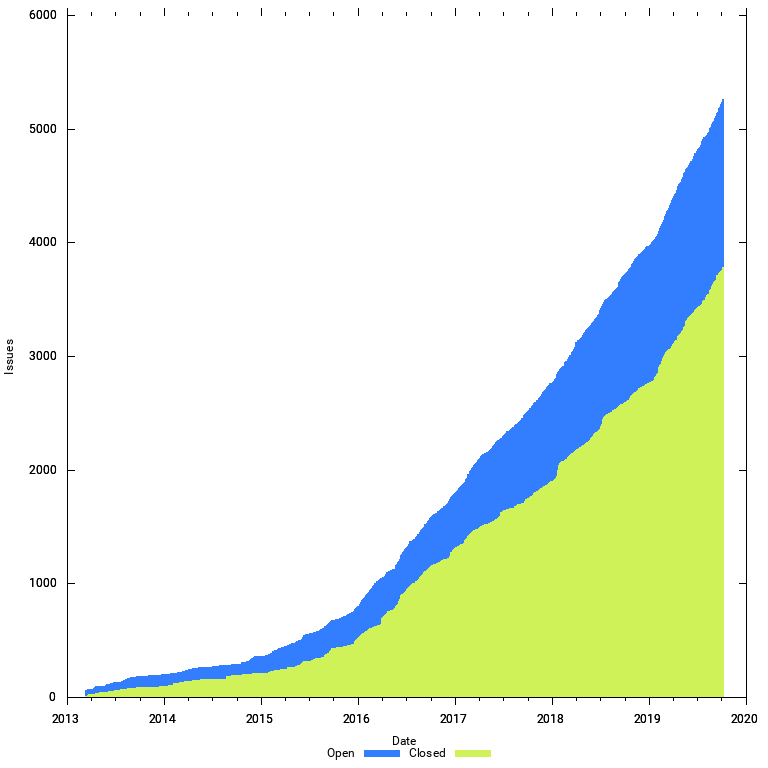
\includegraphics[scale=0.18]{cfd.png}
        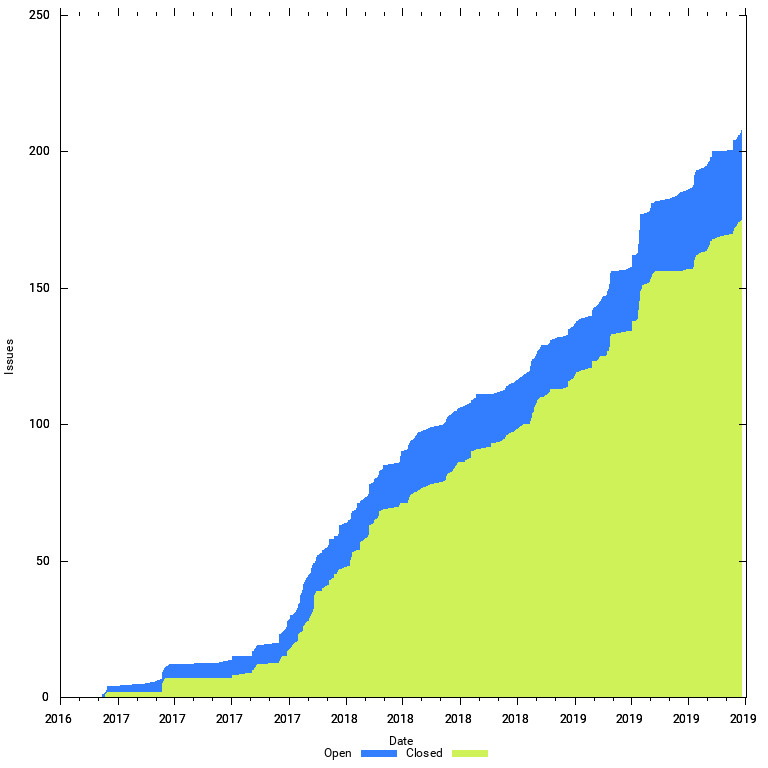
\includegraphics[scale=0.18]{objects-cfd.png}
        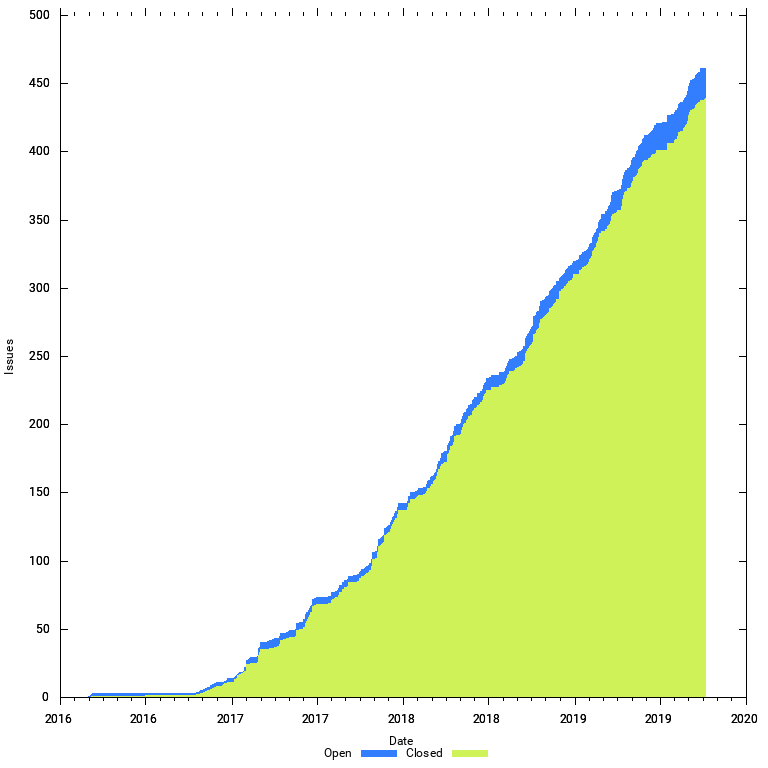
\includegraphics[scale=0.18]{galaxy-cfd.png}
\begin{itemize}
        \item Increase of contributions during 2019 (MISP core, MISP objects and galaxy libraries).
\end{itemize}

\end{frame}

\begin{frame}
        \frametitle{Major outcomes in 2019}
        \begin{itemize}
                \item Improved external tools were created during 2019 such as {\bf misp-dashboard} (4 releases) - a new release is foreseen in the next weeks
                \item The decaying model for indicators described as a academic paper in 2018 is now part of the core MISP software\footnote{\url{https://www.misp-project.org/2019/09/12/Decaying-Of-Indicators.html}}
                \item {\bf All MISP training materials are released as open content}\footnote{\url{https://github.com/MISP/misp-training}} and contain more than 36 hours of training (e.g. MISP usage, administration, OSINT analysis and collection,  building sharing communities)
                        \begin{itemize}
                                \item Source code is available and translation(s)/contribution(s) are welcome
                        \end{itemize}
        \end{itemize}
\end{frame}

\begin{frame}
        \frametitle{MISP object templates}
        \begin{itemize}
                \item From 89 (in 2018) to 147 (in 2019) object templates were added from many external contributors
                \item Object templates include updated {\bf telecom objects} (such as SS7, GTP, Diameter or IMSI-catcher output), {\bf cyber security objects}, {\bf security objects} (such as vehicule, interpol-notice)
                \item Objects are more and more used in different sharing communities and take over simple attributes in MISP to offer better contextualisation
        \end{itemize}
\end{frame}



\begin{frame}
        \frametitle{Conclusion}
        \begin{itemize}
                \item 2019 was a busy and successful year for the MISP project
                \item The 2-year CEF grant was a bootstrap to improve MISP to its next level
                \item New partnerships and projects are ongoing in 2020-2021 (such as the CEF VARIoT project or H2020 Enforce)
                \item As the MISP project becomes larger, we improve the structure of the project (misp-standard.org is the first step)
        \end{itemize}
\end{frame}

